\documentclass{ximera}
\author{Jim Talamo}
\newcommand{\RR}{\mathbb R}
\renewcommand{\d}{\,d}
\newcommand{\dd}[2][]{\frac{d #1}{d #2}}
\renewcommand{\l}{\ell}
\newcommand{\ddx}{\frac{d}{dx}}
\newcommand{\dfn}{\textbf}
\newcommand{\eval}[1]{\bigg[ #1 \bigg]}


\title[Dig-In:]{Remainders for Geometric and Telescoping Series}

\outcome{Work with the remainder for a convergent geometric series.}
\outcome{Work with the remainder for a convergent telescoping series.}
\outcome{Estimate the value of a convergent series using the sequence of partial sums.}
\outcome{Explain the relationship between the remainder of a convergent series and the sequence of partial sums.}

\begin{document}
\begin{abstract}
For a convergent geometric series or telescoping series, we can find the exact error made when approximating the infinite series using the sequence of partial sums.
\end{abstract}
\maketitle

We've seen that if we have a \emph{convergent} series , we can approximate its value by summing only finitely many of its terms.  For instance if we consider $\sum_{k=1}^{\infty} a_k$, we can split the series up.

\begin{image}
  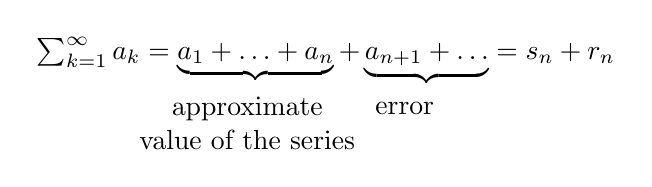
\begin{tikzpicture}
        \node at (0,0) {
          $ \sum_{k=1}^{\infty} a_k=\underbrace{a_1+\ldots +a_n}+ \underbrace{a_{n+1}+ \ldots} = s_n+r_n$};
        \node at (1,-.6) { error};
       
        \node at (-1,-.6) {approximate };
        \node at (-1,-1) {value of the series };
                
      \end{tikzpicture}
  \end{image}

We thus have two important sequences associated with any convergent series $\sum_{k=n_0}^{\infty} a_k$.

\begin{itemize}
\item $\{s_n\}_{n=n_0}$ : The term $s_n$ is found by adding all terms up to and including $a_n$ and tells us the approximate value of the infinite series $\sum_{k=n_0}^{\infty} a_k$.
 \item $\{r_n\}_{n=1}$ : The term $r_n$ is the error made by approximating the infinite series $\sum_{k=n_0}^{\infty} a_k$ by $s_n$ (that is, by approximating $\sum_{k=n_0}^{\infty} a_k$ by $\sum_{k=n_0}^n a_k$).
\end{itemize}

When we have an explicit formula for $s_n$, we can determine an exact formula for the error term $r_n$; we simply use the relationship $\sum_{k=n_0}^{\infty} a_k =   s_n +r_n$.  We can compute $\sum_{k=n_0}^{\infty} a_k$ by taking $\lim_{n \to \infty} s_n$ and subtract $s_n$ form both sides to obtain the formula for $r_n$.  We have seen that there are two special types of series when we can find such a description for $\{s_n\}_{n=1}$, which we explore below.

   
%%%%%%%%%%%%%%%%%%%%%%%%%%%%%%%%%%%%%%%%%%%%%%%%%%%%%%%%%%%%%%%%%%%%%

\section{Remainders for geometric series}
Recall that a series $\sum_{k=n_0}^{\infty} a_k$ is geometric if for each $n\geq n_0$, there are constants $a$ and $r$ for which $a_n = ar^n$.  We also know precisely when such series converge.

\begin{theorem}
\index{series!geometric}\index{geometric series}\index{geometric series!convergence}\index{geometric series!divergence}
  The geometric series $\sum_{k= k_0}^\infty a \cdot r^k$ 
  
  \begin{itemize} 
  \item converges to $\frac{ar^{k_0}}{1-r}$ when $|r| < 1$.
  \item diverges if $|r| \geq 1$.  
  \end{itemize}
  \end{theorem}
  
En route to establishing this result, we determined that when $n_0=0$,

\[
s_n = \sum_{k=0}^n ar^k = \frac{a-ar^{n+1}}{1-r}.
\]  

We can use this to find a formula for $r_n$ when $|r|<1$.

\begin{example}
Consider the series $\sum_{k=0}^{\infty} 2\left(\frac{1}{3}\right)^k$.  We find an explicit formula for $r_n$.

\begin{explanation}
First, note that the series converges, so we may define the sequence of remainders.  To fin a formula for $r_n$, we first a formula for $s_n$.  Since this is a geometric series with $a= \answer{2}$ and $r = \answer{\frac{1}{3}}$, we find that 

\begin{align*}
s_n &= \frac{2-2\left(\frac{1}{3}\right)^{n+1}}{1-\frac{1}{3}} \\
&= \left[2-2\left(\frac{1}{3}\right)^{n+1}\right] \cdot \frac{3}{2} \\
&= \cancel{2} \cdot \frac{3}{\cancel{2}}- \cancel{2}\left(\frac{1}{3}\right)^{n+1} \cdot \frac{3}{\cancel{2}}\\
s_n &= 3-\left(\frac{1}{3}\right)^{\answer{n}}
\end{align*}

We can also compute that $\lim_{n \to \infty} s_n = \answer{3}$ (either directly from the above or from the convergence result for geometric series).  We can now find a formula for $r_n$.

\begin{align*}
\sum_{k=0}^{\infty} 2\left(\frac{1}{3}\right)^k &= s_n + r_n \\
3 &= 3-\left(\frac{1}{3}\right)^{n} + r_n \\
r_n &=\answer{\left(\frac{1}{3}\right)^{n}} . \\
\end{align*}

\end{explanation}
\end{example}

Armed with an explicit formula for both $s_n$ and $r_n$, we can arrange the first several terms in each sequence in a table.

\begin{example}
By using the formulas for $s_n$ and $r_n$, fill in the table below.  

\begin{center}
\begin{tabular}{c | c | c | c | c | c }
n& $0$ & $1$ & $2$ & $3$ & $10$ \\ [2 ex]
\hline
$s_n$ & $0$ &$ \answer{\frac{8}{3}}$ & $\answer{\frac{26}{9}}$ & $\frac{80}{27}$ & $\frac{177146}{59049}$ \\ [2 ex]
\hline
$r_n$ & $3$ & $\answer{\frac{1}{3}}$ & $\frac{1}{9}$ & $\answer{\frac{1}{27}}$ & $\frac{1}{59049}$
\end{tabular}
\end{center}

Note that for each value of $n$, we have that $s_n + r_n = \answer{3}$, which should not be surprising!  We thus see that for each $n$, $s_n$ gives the approximate value of the series, while $r_n$ gives the error of this approximation.  Furthermore, notice something nice here; $\{r_n\}_{n=0}$ is a \wordChoice{\choice{increasing}\choice[correct]{decreasing}} sequence, meaning that as we use more terms to approximate the infinite series, the error becomes smaller! 
\end{example}

In most applications, we will only want to determine the value of a convergent series to a specified degree of accuracy.  While we can compute the exact value of the series in the last example, this is not always the case.  To gain some insight, we will use the previous exercise to estimate the series  $\sum_{k=0}^{\infty} 2\left(\frac{1}{3}\right)^k$ to within $.001$ of its exact value.  To do this, we will add finitely many terms and verify how good this approximation is.

\begin{example}
What is the smallest value of $N$ so the series $\sum_{k=0}^{N} 2\left(\frac{1}{3}\right)^k$ is within $.001$ of the exact value of $\sum_{k=0}^{\infty} 2\left(\frac{1}{3}\right)^k$?  For this choice of $N$, what is $\sum_{k=0}^{N} 2\left(\frac{1}{3}\right)^k$ to four decimal places?

\begin{explanation}
We are being asked to use finite sum $s_N = 2+2\left(\frac{1}{3}\right)+\ldots + 2\left(\frac{1}{3}\right)^N$ to approximate the infinite series $\sum_{k=0}^{\infty} 2\left(\frac{1}{3}\right)^k$.   We have established that the error in this approximation will be $r_N = \left(\frac{1}{3}\right)^{n}$.  Thus, we may find $N$ by setting $\left(\frac{1}{3}\right)^{N} <.001$ and solving for $N$.

\begin{align*}
r_N  \left(\frac{1}{3}\right)^{N} &\leq .001 \\
\ln \left(\frac{1}{3}\right)^{N} &\leq \ln(.001) \\
N \ln \left(\frac{1}{3}\right) &\leq \ln(.001) \\
N &\geq \frac{\ln(.001)}{\ln \left(\frac{1}{3}\right)} \textrm{(note the sign changes since } \ln \left(\frac{1}{3}\right) \textrm{ is negative).}\\
\end{align*}

Using a calculator (or other technology), we compute to one decimal place that $N \geq \answer[tolerance=.1]{6.3}$.  This means that we need to sum up to at least $N=6.3$, meaning that we will need to use $N=7$.

We thus know that $\sum_{k=0}^7 2\left( \frac{1}{3}\right)^k$ will approximate $ \sum_{k=0}^\infty 2\left( \frac{1}{3}\right)^k$ to within at least $.001$ of its exact value.  To verify this, compute $\sum_{k=0}^7 2\left( \frac{1}{3}\right)^k$ to four decimal places.

\[
\sum_{k=0}^7 2\left(\frac{1}{3}\right)^k = 2+2\left(\frac{1}{3}\right)+2\left(\frac{1}{3}\right)^2+\ldots+ 2\left(\frac{1}{3}\right)^7 \approx \answer{2.9995}.
\]

Noting that the exact value of $\sum_{k=0}^\infty 2\left( \frac{1}{3}\right)^k$ is $\answer{3}$, we see that $s_7$ \wordChoice{\choice[correct]{approximates}\choice{does not approximate}} the exact value to within $.001$.
\end{explanation}
\end{example}

%%%%%%%%%%%%%%%%%%%%%%%%%%%%%%%%%%%%%%%%%%%%%%%%%%%%%%%%%%%%%%%%%%%%%%

\section{Remainders for telescoping series}
The other type of series for which we could find an explicit formula for $s_n$ are \emph{telescoping series}.

 \begin{example}
Consider the series $\sum_{k=2}^{\infty} \frac{4}{k^2-1}$.  We find an explicit formula for $r_n$.

\begin{explanation}
We can determine that the series converges by finding an explicit formula for $s_n$ if we first do a partial fraction decomposition (which makes sense to try since we can factor the denominator).

\[
 \frac{4}{k^2-1} = \frac{\answer{2}}{k-1}-\frac{\answer{2}}{k+1}
\]

We can write out several terms in the sequence of partial sums.

\begin{align*}
a_2&= \frac{2}{1}-\frac{2}{3} & s_2&= \frac{2}{1}-\frac{2}{3} \\
a_3&= \frac{2}{2}-\frac{2}{4} & s_3&= \frac{2}{1}+\frac{2}{2}-\frac{2}{3}-\frac{2}{4} \\
a_4&= \frac{2}{3}-\frac{2}{5} & s_4&= \frac{2}{1}+\frac{2}{2}-\frac{2}{4}-\frac{2}{5} \\
a_5&= \frac{2}{4}-\frac{2}{6} & s_5&= \frac{2}{1}+\frac{2}{2}-\frac{2}{5}-\frac{2}{6} \\
a_6&= \frac{2}{5}-\frac{2}{7} & s_6&= \frac{2}{1}+\frac{2}{2}-\frac{2}{6}-\frac{2}{7} \\
\end{align*}

From pattern recognition, we see that $s_n = 3 - \frac{2}{n} - \frac{2}{n+1}$, and we can explicitly take a limit to find $\lim_{n \to \infty} s_n = \answer{3}$, so $\sum_{k=2}^{\infty} a_k$ \wordChoice{\choice[correct]{converges to $3$}\choice{diverges}}.

With both the value of $\sum_{k=2}^{\infty} a_k$ and a formula for $s_n$, we may find a formula for $r_n$.  

\begin{align*}
\sum_{k=0}^{\infty}  \frac{4}{k^2-1} &= s_n + r_n \\
3 &= 3- \frac{2}{n} - \frac{2}{n+1} + r_n \\
r_n &= \frac{2}{n} + \frac{2}{n+1} \\
\end{align*}

\end{explanation}

By using the formula for $r_n$, what error is made by approximating $\sum_{k=2}^{\infty} \frac{4}{k^2-1}$ by $\sum_{k=2}^{100} \frac{4}{k^2-1}$?

\begin{explanation}
To find the error, we need to find $r_{\answer{100}}$.  Using the formula from the last part, we find

\begin{align*}
r_{100} &= \frac{2}{\answer{100}} + \frac{2}{\answer{101}} \\
&= \answer[tolerance=.001]{.0398} \qquad \textrm{(to four decimal places)}
\end{align*}

We thus expect that the error made by approximating $\sum_{k=2}^{\infty} \frac{4}{k^2-1}$ by $\sum_{k=2}^{100} \frac{4}{k^2-1}$ is (to four decimal places) $\answer{.0398}$.

\end{explanation}
\end{example}

\begin{remark}
A computer can evaluate $\sum_{k=2}^{100} \frac{4}{k^2-1}$ very quickly, and it will give us that, to four decimal places, $\sum_{k=2}^{100} \frac{4}{k^2-1} = 2.9602$.  We thus have that $s_{100}+r_{100} = 2.9602+.0398 =3$, as expected, since the value of the series will be the approximate value plus the error.
\end{remark}

\section{Conclusion}
When we have a convergent geometric or telescoping series, we can find an explicit formula for $s_n$, which allows us to find the exact value of the series as well as an explicit formula for the terms in the sequence of remainders.  We have then seen how the terms in the sequence of remainders give the error made by approximating the infinite series by a finite sum.

One very important point to remember is that the calculations in this section are possible because we consider \emph{convergent} series; remember it is not possible to define a sequence of remainders for a divergent series!

\begin{question}
Select all of the series below for which it is possible to define a sequence of remainders.

\begin{selectAll}
\choice[correct]{$\sum_{k=2}^{\infty} \left(\frac{2}{9}\right)^k$}
\choice{$\sum_{k=1}^{\infty} \left(\frac{4}{3}\right)^k$}
\choice{$\sum_{k=1}^{\infty} \frac{2k}{4k+1}$}
\end{selectAll}

\begin{feedback}
We can only define the sequence of remainders for convergent series.

\begin{itemize}
\item $\sum_{k=2}^{\infty} \left(\frac{2}{9}\right)^k$ is a convergent geometric series.
\item $\sum_{k=1}^{\infty} \left(\frac{4}{3}\right)^k$ is a divergent geometric series.
\item $\sum_{k=1}^{\infty} \frac{2k}{4k+1}$ diverges by the divergence test.
\end{itemize}
\end{feedback}

\end{question}

\end{document}
